
\section*{Instructions and Help}

\textbf{Please remove this part and the sample references before submitting your homework.}

Read the general homework instructions available on the course homepage before starting to write the report.

Here are some additional guidelines how to write a homework report.
\begin{itemize}
 \item Fill in name and personal number of all group members.
 \item Each group uploads one file on Canvas within the deadline specified on the \texttt{Homework} page.
 \item This report should contain solutions to the first 19 tasks in Homework~3.
 \item This file needs to be one zip file with name \texttt{name1-name2-name3-name4-HW3.zip}, where \texttt{name1,...,name4} are the last names of the authors. The zip file should contain 4 files: one pdf file named \texttt{name1-name2-name3-name4-HW3.pdf} and three controller files \texttt{OwnVariables.c}, \texttt{Controller.c} and
 \texttt{RenewControllerState.c}.
 \item Do not copy the task descriptions and use the structure below.
 \item Do not include code unless the task explicitly states so.
 \item Motivate your answers well and how you derived them, but be concise.
 \item The number of points is not necessarily related to much you need to write for task.
 \item Put references in the end if any.
 \item Do not include plots from the Simulink scope (color on black background) but export the data to Matlab for plotting.
 \item Include graphics directly in the text and not in a Figure environment, as you normally would. That makes it easier to correct the report.
 \item There is plenty of material available how to use Latex. Use a search engine of your choice to learn more.
\end{itemize}

Here are some examples how to use Latex:
\begin{itemize}
 \item An equation with a reference \eqref{eq_sample} to it
 \begin{equation}
  \dot{x} = \frac{3}{4} x. \label{eq_sample}
 \end{equation}
 \item A multi-line equations with a reference to it
 \begin{align*}
  \hat{x} &= x - y\\
  \alpha &= x + \gamma.
 \end{align*}
 \item An equation in text: $\Phi = \int\limits_{0}^{h} \mathrm{e}^{A\tau} d \tau$.
 \item An image
 \begin{center}
  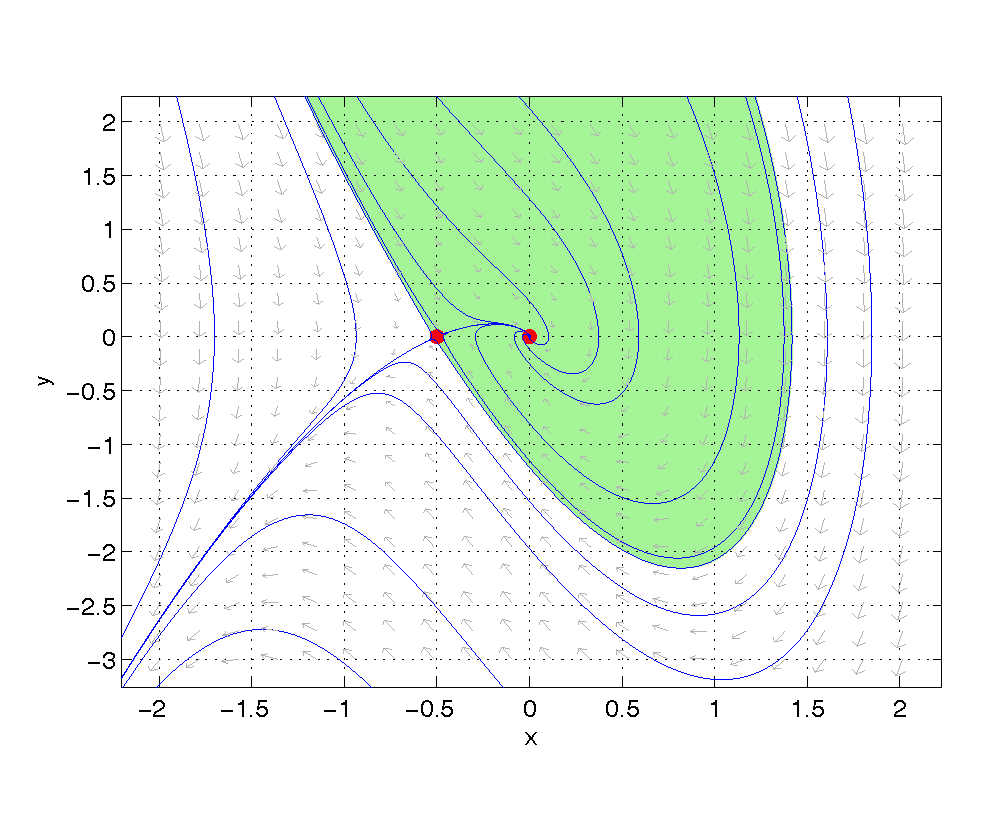
\includegraphics[width = 0.8\textwidth]{Phase_portrait_with_regionmark}
 \end{center}
 \item A table

 \begin{tabular}{@{\vrule height 10.5pt depth4pt  width0pt}|c|c|c|c|}
    \hline
     $-2.46$ & $0$ & $-1.73$ & $0$ \\ \hline
     $0$ & $-2.553$ & $0$ & $2.774$ \\ \hline
     $0$ & $6.172$ & $-10$ & $7.333$ \\ \hline
     $1.767$ & $-0.357$ & $5.714$ & $-6.074$ \\ \hline
  \end{tabular}
  \item A citation \cite{Oetiker:2008:TheNotSoShortIntroductiontoLaTeXe}
  \item Display something exactly as it is written: \verb|\frac{1}{2}_|
  \item Basic formating: \textbf{bold}, \textit{italics}, \texttt{typewriter}
\end{itemize}
